\documentclass{article}
\usepackage{bm}
\usepackage{amsmath}
\usepackage{graphicx}
\usepackage{mdwlist}
\usepackage[colorlinks=true]{hyperref}
\usepackage{geometry}
\usepackage{kotex}
\geometry{margin=1in}
\geometry{headheight=2in}
\geometry{top=2in}
\usepackage{palatino}
%\renewcommand{\rmdefault}{palatino}
\usepackage{fancyhdr}

\newcommand{\red}[1]{{\color{red} #1}}
\newcommand{\blue}[1]{{\color{blue} #1}}
\newcommand{\orange}[1]{{\color{orange} #1}}
\newcommand{\purple}[1]{{\color{purple} #1}}

%\pagestyle{fancy}
\rhead{}
\lhead{}
\chead{%
  {\vbox{%
      \vspace{2mm}
      \large
      Hardware System Design 4190.309A\hfill
\\
      Seoul National University
      \\[4mm]
      \textbf{Practice \#11. DMA (Direct Memory Access)}\\
      \textbf{Jiwon Lee, Sangjun Son}
    }
  }
}

%%%%%%%%%%%%%%%%%%%%%%%
\usepackage{xcolor}
\usepackage{listings}
\definecolor{vgreen}{RGB}{104,180,104}
\definecolor{vblue}{RGB}{49,49,255}
\definecolor{vorange}{RGB}{255,143,102}

\lstdefinestyle{c-style}
{
    language=C,
    basicstyle=\scriptsize\ttfamily,
    keywordstyle=\color{vblue},
    identifierstyle=\color{black},
    commentstyle=\color{vgreen},
    numbers=left,
    numberstyle=\tiny\color{black},
    numbersep=10pt,
    tabsize=8,
    moredelim=*[s][\colorIndex]{[}{]},
    literate=*{:}{:}1
}
\lstdefinestyle{python-style}
{
    language=Python,
    basicstyle=\scriptsize\ttfamily,
    keywordstyle=\color{vblue},
    identifierstyle=\color{black},
    commentstyle=\color{vgreen},
    numbers=left,
    numberstyle=\tiny\color{black},
    numbersep=10pt,
    tabsize=8,
    moredelim=*[s][\colorIndex]{[}{]},
    literate=*{:}{:}1
}

\makeatletter
\newcommand*\@lbracket{[}
\newcommand*\@rbracket{]}
\newcommand*\@colon{:}
\newcommand*\colorIndex{%
    \edef\@temp{\the\lst@token}%
    \ifx\@temp\@lbracket \color{black}%
    \else\ifx\@temp\@rbracket \color{black}%
    \else\ifx\@temp\@colon \color{black}%
    \else \color{vorange}%
    \fi\fi\fi
}
\makeatother

\usepackage{trace}
%%%%%%%%%%%%%%%%%%%%%%%

\usepackage{paralist}

\usepackage{todonotes}
\setlength{\marginparwidth}{2.15cm}

\usepackage{tikz}
\usetikzlibrary{positioning,shapes,backgrounds}

\begin{document}

\pagestyle{fancy}

\section*{Goal}

\begin{itemize*}
\item Implement convolution lowering in C++.
\item Integrate convolution lowering into the pretrained model (CNN).
\begin{itemize*}
\item On MNIST dataset as Figure~\ref{fig1}.
\end{itemize*}
\end{itemize*}
\begin{figure}[ht]
	\centering
	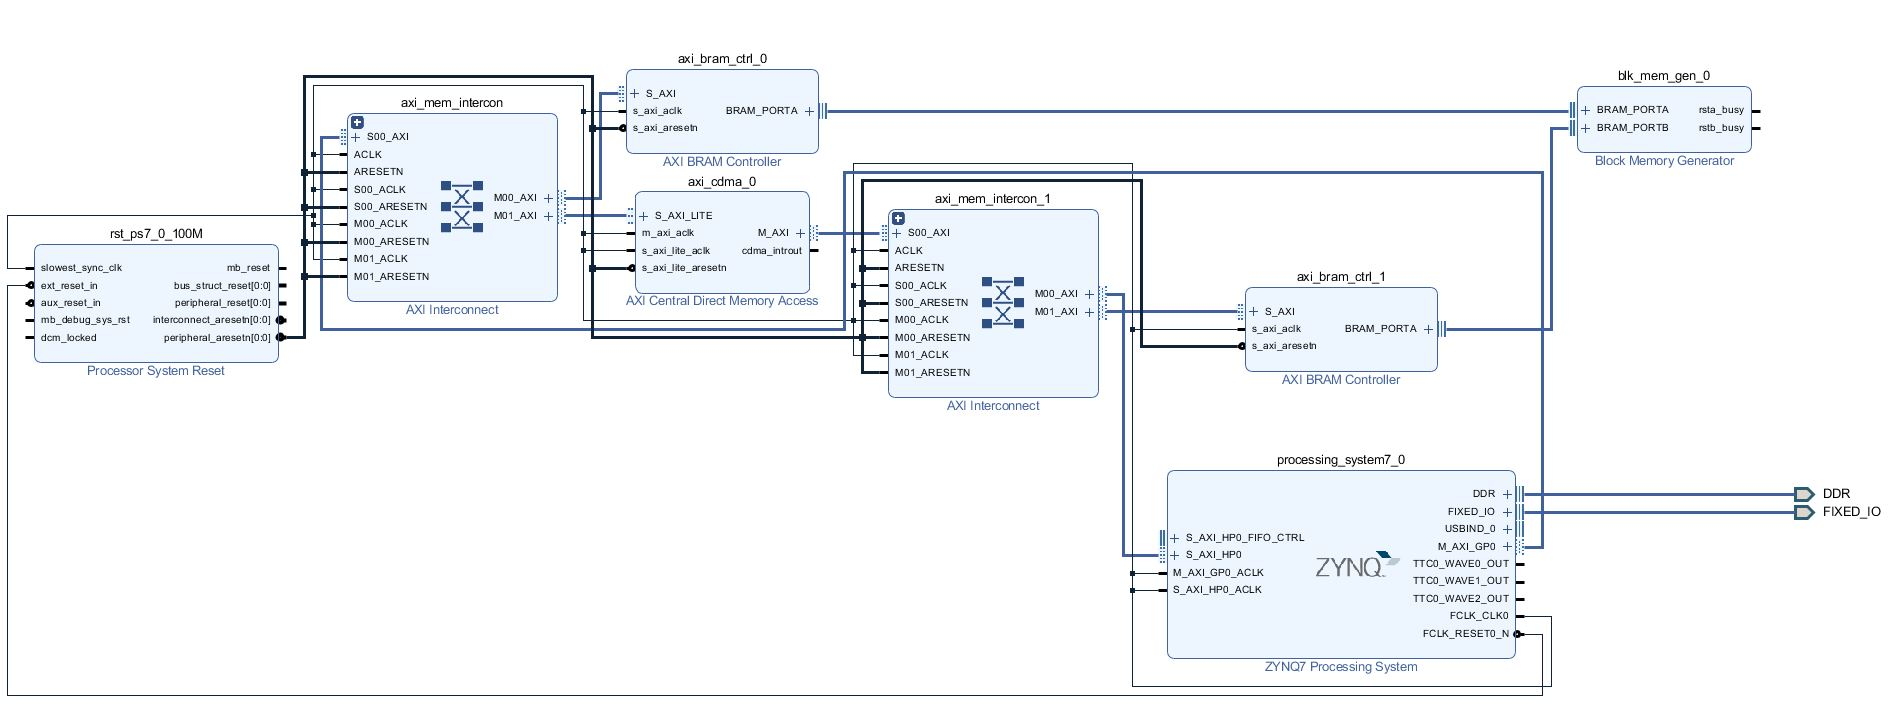
\includegraphics[width=1\textwidth]{fig/overview.jpg}
\caption{Overview of DMA with BRAM.}
\label{fig1}
\end{figure}

\section{Implementation}
지난 Lab 2에서 구현한 Multi-Layer Perceptron으로 MNIST 숫자를 예측하는 프로젝트의 연장선에서 CNN 모델 또한 구현하기 위해 Matrix-Matrix Multiplication과 Convolution Lowering을 구현하고 이를 Zedboard CPU 위에서 수행하는 실험을 한다. \\

MLP 모델의 경우 28 x 28 크기의 숫자 이미지이며 이를 벡터화 하여 여러 Layer를 거쳐 마지막에 output layer에 10개의 숫자 중 나타날 확률을 학습하게 된다. 행렬과 벡터 곱셈이 매우 크므로 공간이나 시간적 복잡도를 최적화하기 위해서는 Tiling method를 사용하였으며 이 방법을 CNN 모델의 행렬 곱셈에서도 사용하게 된다. 행렬과 벡터 또는 행렬과 행렬을 일정한 크기로 나누어 가속기를 통해 쓰레드를 나누어 빠른 연산 속도를 가능하게 한다. \\


결론적으로 이번 실습에서 구현하고 검증해야 하는 Operation은 다음과 같이 세 가지이다.
\begin{enumerate}
    \item \textit{Matrix-Vector Multiplication}\\
    Block operation (Tiling Method)을 활용한 행렬 벡터 연산
    \item \textit{Matrix-Matrix Multiplication}\\
    Block operation (Tiling Method)을 활용한 행렬 행렬 연산
    \item \textit{Convolution Lowering} \\
    Image와 Convolution Filter 데이터를 재정렬하여 Matrix Multiplication로 바꾸는 행렬화 작업~\cite{chellapilla2006high, chetlur2014cudnn}
\end{enumerate}

\subsection{Matrix-Vector Multiplication}
\label{sec:mv}
행렬 벡터 연산을 수행할 때는 작은 크기의 행렬 벡터 연산 (Tiling)으로 축소 대응시켜 계산을 하게 되는데 이 때 자주 사용되는 함수가 block operation이다. 함수를 사용하기 위해서 중간 중간에 \texttt{data\_}라는 데이터 중간 저장소를 통해 곱셈에 사용될 행렬과 벡터를 fetching 하고 연산된 output vector를 덮어쓰는 과정을 반복하게 된다. 코드에 대한 자세한 설명은 Lab 2를 참고하면 된다~\cite{lab2}.

\subsection*{\texttt{FPGA::largeMV}}
\begin{lstlisting}[style={c-style}]
void FPGA::largeMV(const float* large_mat, const float* input, float* output, int num_input, int num_output)
{
  float* vec = this->vector();
  float* mat = this->matrix();

  // 0) Initialize output vector		
  for(int i = 0; i < num_output; ++i)
    output[i] = 0;

  for(int i = 0; i < num_output; i += m_size_)
  {
    for(int j = 0; j < num_input; j += v_size_)
    {			
      // 0) Initialize input vector
      int block_row = min(m_size_, num_output-i);
      int block_col = min(v_size_, num_input-j);
            
      // 1) Assign a vector
      for (int col = 0; col < block_col; col++)
        data_[col] = input[j + col];
      for (int col = block_col; col < v_size_; col++)
        data_[col] = 0;

      // 2) Assign a matrix
      for (int row = 0; row < block_row; row++)
        for (int col = 0; col < block_col; col++)
          data_[(row+1)*v_size_ + col] = large_mat[(i+row)*num_input + (j+col)];


      // 3) Call a function `blockMV() to execute MV multiplication
      const float* ret = this->blockMV();

      // 4) Accumulate intermediate results
      for(int row = 0; row < block_row; ++row)
        output[i + row] += ret[row];
    } 
  }
}
\end{lstlisting}

\subsection{Matrix-Matrix Multiplication}
Section~\ref{sec:mv}과 마찬가지로 Tiling Method으로 축소 대응시켜 계산을 하면 된다. 함수를 사용하기 위해서 중간 중간에 \texttt{data\_M}라는 데이터 중간 저장소를 통해 곱셈에 사용될 2개의 행렬을 fetching 하고 연산된 output vector를 덮어쓰는 과정을 반복하게 된다. 

\begin{figure}[htb!]
	\centering
	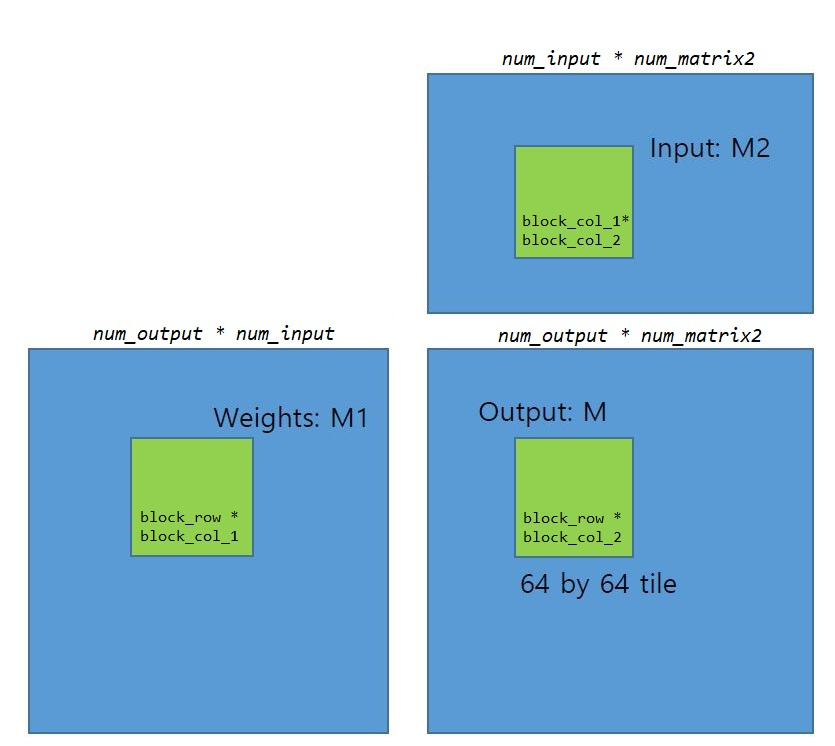
\includegraphics[width=0.6\textwidth]{fig/mm.jpg}
\caption{Block operation에 사용되는 행렬의 곱셈 연산 부분, 파란색 행렬을 곱셈하기 위해 Tiling Method으로 쪼개었을 때 연두색 행렬끼리의 곱셈으로 Output Matrix를 채워나갈 수 있다. 위 예시는 쪼개는 단위인 \texttt{v\_size}가 64이다.}
\label{fig3}
\end{figure}

Figure~\ref{fig3}에서 볼 수 있듯이 기본적으로 \texttt{v\_size} 간격으로 작은 Block operation을 수행하지만 행렬의 가로, 세로 크기가 항상 \texttt{v\_size}의 배수가 아니므로 경계부분에서의 예외처리를 위해 Block 사이즈를 나타내는 변수 \texttt{block\_row},  \texttt{block\_col\_1}, \texttt{block\_col\_2}를 도입한다.

\subsection*{\texttt{FPGA::largeMM}}
\begin{lstlisting}[style={c-style}]
void FPGA::largeMM(const float* weight_mat, const float* input_mat, float* output, 
		   int num_input, int num_output, int num_matrix2)
{
  float* m1 = this->matrix_M1();
  float* m2 = this->matrix_M2();

  // 0) Initialize output vector		
  for(int i = 0; i < num_output*num_matrix2; ++i)
    output[i] = 0;

  for(int i = 0; i < num_output; i += v_size_)
  {
    for(int j = 0; j < num_input; j += v_size_)
    {
      for(int k = 0; k < num_matrix2; k += v_size_)
      {
        // 0) Initialize input vector
        int block_row = min(v_size_, num_output-i);
        int block_col_1 = min(v_size_, num_input-j);
        int block_col_2 = min(v_size_, num_matrix2-k);

        // 1) Assign a m1
        for (int row = 0; row < block_row; row++) {
          for (int col = 0; col < block_col_1; col++)
            data_M[row*v_size_ + col] = weight_mat[(i+row)*num_input + (j+col)];
          for (int col = block_col_1; col < v_size_; col++)
            data_M[row*v_size_ + col] = 0;
      	}
        for (int l = block_row*v_size_; l < m1_size_; l++)
            data_M[l] = 0;

        // 2) Assign a m2
        for (int row = 0; row < block_col_1; row++) {
          for (int col = 0; col < block_col_2; col++)
            data_M[m1_size_ + row*v_size_ + col] = input_mat[(j+row)*num_matrix2 + (k+col)];
          for (int col = block_col_2; col < v_size_; col++)
            data_M[m1_size_ + row*v_size_ + col] = 0;
      	}
        for (int l = block_col_1*v_size_; l < m2_size_; l++)
            data_M[m1_size_ + l] = 0;

        // 3) Call a function `blockMM() to execute Matrix matrix multiplication
        const float* ret = this->blockMM();

        // 4) Accumulate intermediate results
        for(int n = 0; n<block_row; ++n)
        {
          for(int m = 0; m<block_col_2; ++m)
          {
            output[(i + n) + (k + m)*num_output] += ret[n*v_size_ + m];
          }
        }
      }
    } 
  }
}
\end{lstlisting}

\begin{itemize*}
\item Block OP를 수행할 부분인 Weight Matrix를 \texttt{data\_M}에 먼저 넣는다 (24 라인).
\item 이 행렬의 크기는 \texttt{block\_row} * \texttt{block\_col\_1} 이므로 첫 번째 행렬 부분에 해당하는 \texttt{m1\_size\_} 중 사용하지 않는 부분은 모두 0으로 초기화한다 (26-29 라인).
\begin{itemize*}
\item 그렇지 않다면 전 step에서 사용되었던 벡터 값이 잘못된 연산 결과를 초래할 수 있기 때문이다~\cite{lab2}.
\end{itemize*}
\item 다음으로 Input Matrix를 \texttt{data\_M}에 넣는다 (34 라인). 
\item 이 행렬의 크기는 \texttt{block\_col\_2} * \texttt{block\_col\_1} 이므로 두 번째 행렬 부분에 해당하는 \texttt{m2\_size\_} 중 사용하지 않는 부분은 모두 0으로 초기화한다 (36-39 라인).
\end{itemize*}

\newpage
\subsection{Convolution Lowering}

\begin{figure}[htb!]
	\centering
	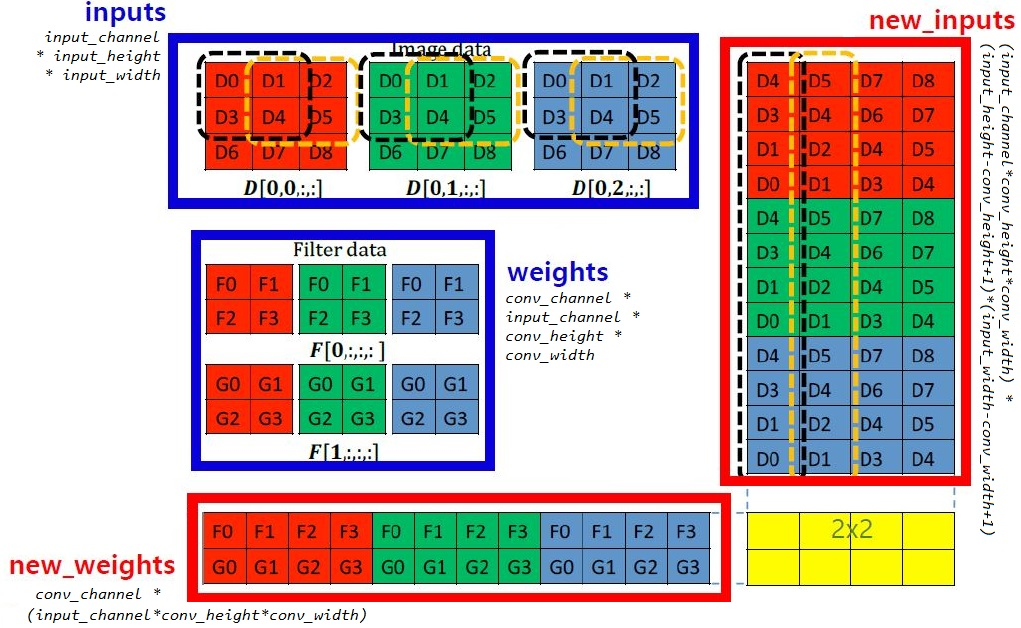
\includegraphics[width=0.9\textwidth]{fig/convlow.jpg}
\caption{Convolution Filter와 Image data에 해당하는 3차원 텐서를 행렬화 시키기 위한 과정을 도식화 한 것~\cite{chetlur2014cudnn, lab9}. 여기서 Convolution Lowering은 \textit{inputs}와 \textit{weight}를 각각 \textit{new\_inputs}와 \textit{new\_weight}로 매핑하는 과정이다.}
\label{fig4}
\end{figure}

Figure~\ref{fig4}를 참조하면 \textit{new\_weight}의 행들은 \textit{weight}의 \texttt{channel}로 나눠지고 각 행은 \texttt{input\_channel} 순서로 \textit{weight} 값이 순서대로 나온다. 아래의 코드의 30-31 라인처럼 \texttt{conv\_channel}, \texttt{input\_channel}, \texttt{conv\_height}, \texttt{conv\_width} 순서대로 for문을 돌면서 \textit{new\_weight} 원소 값을 채워준다. \\

\textit{new\_weight}와 마찬가지로 \textit{new\_inputs}를 구성할 수 있다. 한 Filter가 Input에 방문하는 횟수는 행으로는 \linebreak$\texttt{input\_height} – \texttt{conv\_height} + 1$이고 열의 방향으로는 $\texttt{input\_width} – \texttt{conv\_width} + 1$이 될 것이다. 순서대로 for문을 돌면서 \textit{new\_inputs}의 행열 순서로 채워간다 (38-39 라인).

\subsection*{\texttt{FPGA::convLowering}}
\begin{lstlisting}[style={c-style}]
void FPGA::convLowering(const std::vector<std::vector<std::vector<std::vector<float>>>>& cnn_weights,
    std::vector<std::vector<float>>& new_weights,
    const std::vector<std::vector<std::vector<float>>>& inputs,
    std::vector<std::vector<float>>& new_inputs) {
  /*
   * Arguments:
   *
   * conv_weights: [conv_channel, input_channel, conv_height, conv_width]
   * new_weights: [conv_channel, input_channel*conv_height*conv_width]
   * inputs: [input_channel, input_height, input_width]
   * new_inputs: [input_channel*conv_height*conv_width, (input_height-conv_height+1)*(input_width-conv_width+1)]
   *
   */

  int conv_channel = cnn_weights.size();
  int input_channel = cnn_weights[0].size();
  int conv_height = cnn_weights[0][0].size();
  int conv_width = cnn_weights[0][0][0].size();
  //int input_channel = cnn_weights.size();
  int input_height = inputs[0].size();
  int input_width = inputs[0][0].size();

  // For example,
  // new_weights[0][0] = cnn_weights[0][0][0][0];
  // new_inputs[0][0] = inputs[0][0][0];
  for (int i = 0; i < conv_channel; i++)
    for (int j = 0; j < input_channel; j++)
      for (int k = 0; k < conv_height; k++)
        for (int l = 0; l < conv_width; l++)
          new_weights[i][j*conv_height*conv_width + k*conv_width + l] 
            = cnn_weights[i][j][k][l];

  for (int i = 0; i < input_channel; i++)
    for (int j = 0; j < conv_height; j++)
      for (int k = 0; k < conv_width; k++)
        for (int l = 0; l < input_height-conv_height+1; l++)
          for (int m = 0; m < input_width-conv_width+1; m++)
            new_inputs[i*conv_height*conv_width + j*conv_width + k][l*(input_width-conv_width+1) + m] 
              = inputs[i][j+l][k+m];

}
\end{lstlisting}
\newpage
\section{Result}
구현한 코드를 CPU 상에서 Pre-trained MLP와 CNN network를 사용하여 정확도를 측정해보았다. MLP는 0.97의 정확도를 보였으며 CNN은 MLP보다 높은 0.98에서 1.0의 정확도를 보였다. 아래의 Figure~\ref{fig5}는 Lab 9에서 주어진 \texttt{benchmark.sh}를 수행하였을 때의 결과이다. \\

\begin{figure}[htb!]
	\centering
	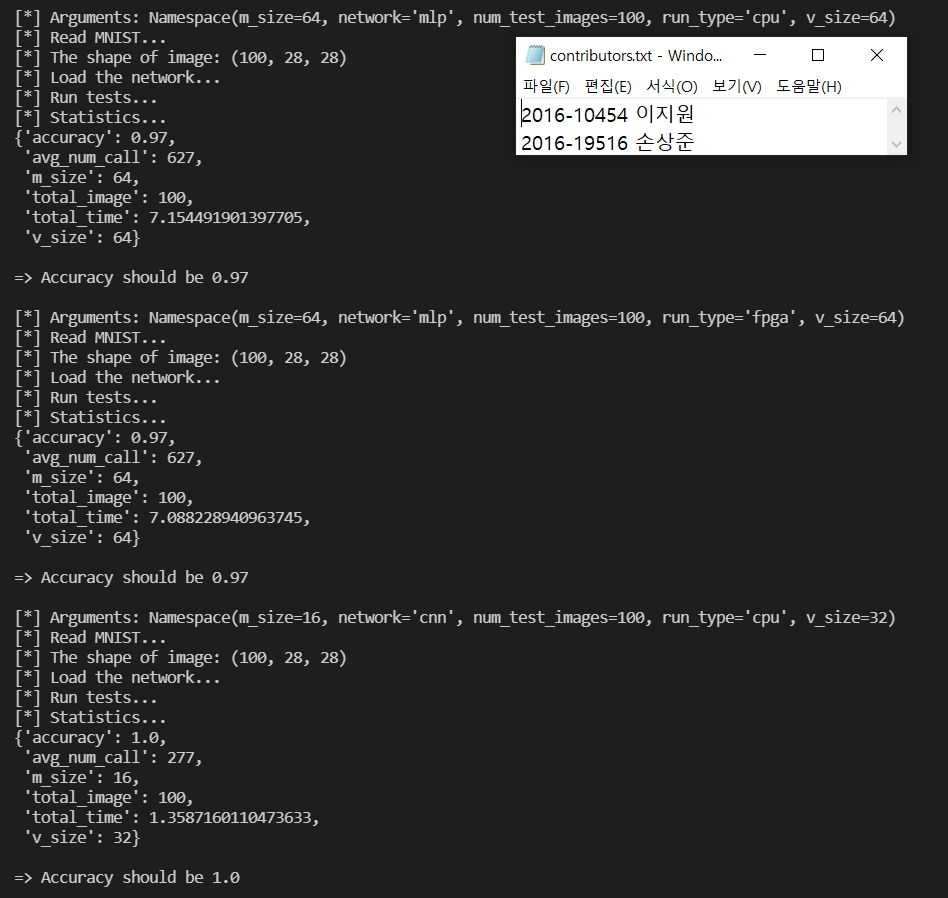
\includegraphics[width=0.8\textwidth]{fig/benchmark results.png}
\caption{Zedboard CPU/FPGA상에서 Pre-trained MLP와 CNN를 사용해 MNIST 데이터셋에 대하여 test 한 결과. \texttt{benchmark.sh}에 포함되지 않은 FPGA CNN은 포함하지 않았다.}
\label{fig5}
\end{figure}

수행 성능에 영향을 미치는 환경변수는 \textit{m\_size},  \textit{v\_size}, \textit{num\_test\_images}가 있으며 네트워크의 종류 또한 변화시키면서 실험을 진행하였다. 기본 값으로는 $\textit{m\_size}=\textit{v\_size}=16$과 $\textit{num\_test\_images}=100$으로 설정하였다. 관측 변수로는 정확도 \textit{accuracy}, 걸리는 시간 \textit{total\_time}, \textit{avg\_num\_call}을 측정하였다. 

\newpage
\begin{table}[htb!]
\renewcommand{\arraystretch}{1.1}
\begin{center}
\begin{tabular}{ |c | c | rrr |} 
 \hline
 Network & Control Variable & \textit{total\_time} & \textit{avg\_num\_call} & \textit{accuracy}  \\ 
 \hline
cnn & num\_test\_images(1) & 0.007s & 553 & 1 \\
cnn & num\_test\_images(10) & 0.067s & 553 & 1 \\
cnn & num\_test\_images(100) & 0.661s & 553 & 1 \\
cnn & num\_test\_images(1000) & 6.635s & 553 & 0.98 \\
cnn & num\_test\_images(10000) & 66.534s & 553 & 0.98 \\
 \hline
cnn & v\_size(1) & 1.589s & 44646 & 1 \\
cnn & v\_size(2) & 0.799s & 9141 & 1 \\
cnn & v\_size(4) & 0.619s & 3050 & 1 \\
cnn & v\_size(8) & 0.56s & 1188 & 1 \\
cnn & v\_size(16) & 0.662s & 553 & 1 \\
cnn & v\_size(32) & 1.34s & 277 & 1 \\
cnn & v\_size(64) & 4.042s & 140 & 1 \\
cnn & v\_size(128) & 37.86s & 71 & 1 \\
 \hline
mlp & num\_test\_images(1) & 0.068s & 9375 & 1 \\
mlp & num\_test\_images(10) & 0.675s & 9375 & 0.9 \\
mlp & num\_test\_images(100) & 6.738s & 9375 & 0.97 \\
mlp & num\_test\_images(1000) & 67.441s & 9375 & 0.92 \\
mlp & num\_test\_images(10000) & 675.352s & 9375 & 0.9159 \\
 \hline
mlp & v\_size(1) & 13.591s & 150000 & 0.97 \\
mlp & v\_size(2) & 9.524s & 75000 & 0.97 \\
mlp & v\_size(4) & 7.34s & 37500 & 0.97 \\
mlp & v\_size(8) & 6.323s & 18750 & 0.97 \\
mlp & v\_size(16) & 6.743s & 9375 & 0.97 \\
mlp & v\_size(32) & 6.537s & 4763 & 0.97 \\
mlp & v\_size(64) & 6.398s & 2419 & 0.97 \\
mlp & v\_size(128) & 6.562s & 1285 & 0.97 \\
 \hline
mlp & m\_size(1) & 8.767s & 149550 & 0.97 \\
mlp & m\_size(2) & 7.663s & 74775 & 0.97 \\
mlp & m\_size(4) & 7.104s & 37425 & 0.97 \\
mlp & m\_size(8) & 6.83s & 18750 & 0.97 \\
mlp & m\_size(16) & 6.745s & 9375 & 0.97 \\
mlp & m\_size(32) & 6.789s & 4787 & 0.97 \\
mlp & m\_size(64) & 6.957s & 2431 & 0.97 \\
mlp & m\_size(128) & 7.502s & 1315 & 0.97 \\
 \hline
\end{tabular}
\caption{ $\textit{m\_size}=\textit{v\_size}=16$과 $\textit{num\_test\_images}=100$로 설정하고 매개 변수를 하나씩 바꿔가면서 측정한 연산 성능 \textit{accuracy}, \textit{total\_time}, \textit{avg\_num\_call} 비교}\label{tab1}
\end{center}
\end{table}

\newpage
\section{Conclusion}
이번 실습에서는 Convolution Lowering을 사용해 CNN 연산을 Matrix Multiplication 연산으로 바꿔보았다. 또한 Lab 2에서 구현한 Matrix Vector Multiplication도 불러와 함께 연산에 사용하였다. MNIST 데이터에 대해서 각각 MLP, CNN으로 inference 한 후 비교해 본 결과 CNN 결과가 조금 더 높은 정확도를 보였다. \\

Convolution Filter의 Weights과 Inputs을 2차원 Matrix를 바꾸는 과정에서 같은 값이 여러 번 사용되어 행렬을 구성하는 것을 확인할 수 있었다. 다시 말하면 더 많은 Memory Allocation을 필요로 하였고 이 부분에서 더 최적화 가능할 것이라고 판단하였다. 또한 실제로 구현되는 CNN을 보면 매개변수로 Stride나 Padding을 넘겨줄 수 있다. 이번 Lab 9에는 이 부분이 빠져 있지만 추가된다면 더욱 더 일반적인 네트워크를 위한 Convolution Lowering을 구현할 수 있을 것이다. \\

\bibliographystyle{plain}
\bibliography{other}

\end{document}
